\chapter{Insert And Retrieve Data }
\section{Insert Data to Firebase Back-end}
\subsection{Create Class Places}
\subitem{
	Create Class of Places and include the place name ,  Location , Describtion , Tags . 
	\begin{figure}[H]
		\centering
		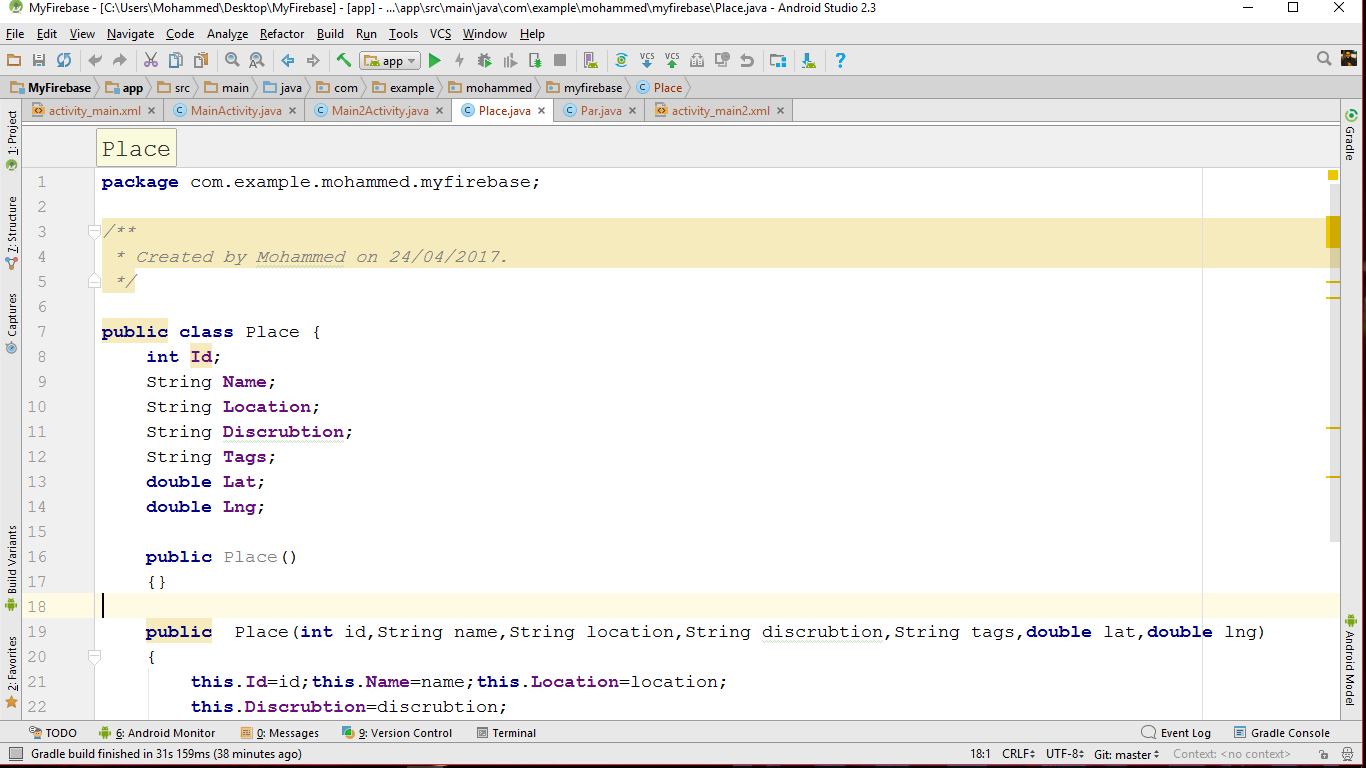
\includegraphics[height=3in]{./TeX_files/pic11}
		\caption[optional caption]{Class of Place}
		\label{Fig:Tobias}
	\end{figure}
	\begin{figure}[H]
		\centering
		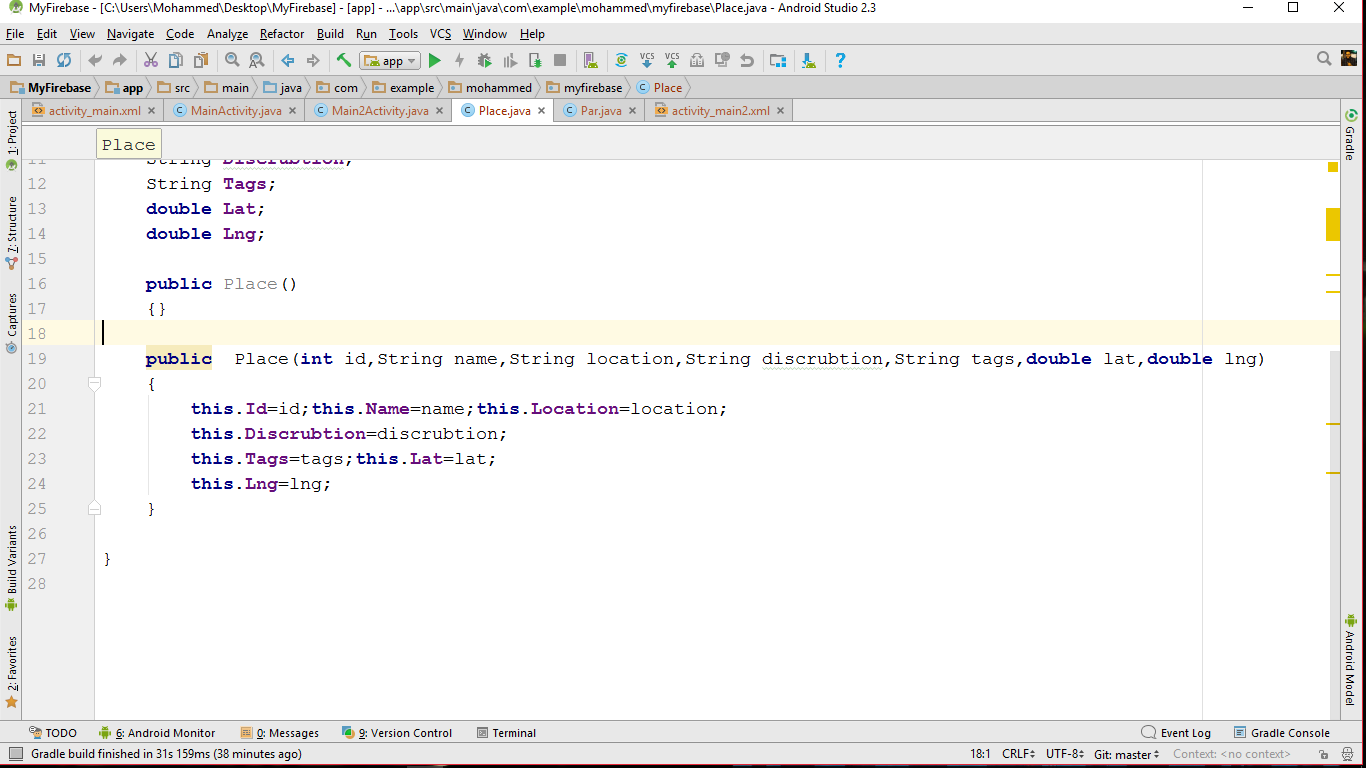
\includegraphics[height=3in]{./TeX_files/pic12}
		\caption[optional caption]{Class of Place}
		\label{Fig:Tobias}
	\end{figure}
	}
\subsection{Design of Layout}
\subitem{
	\begin{figure}[H]
		\centering
		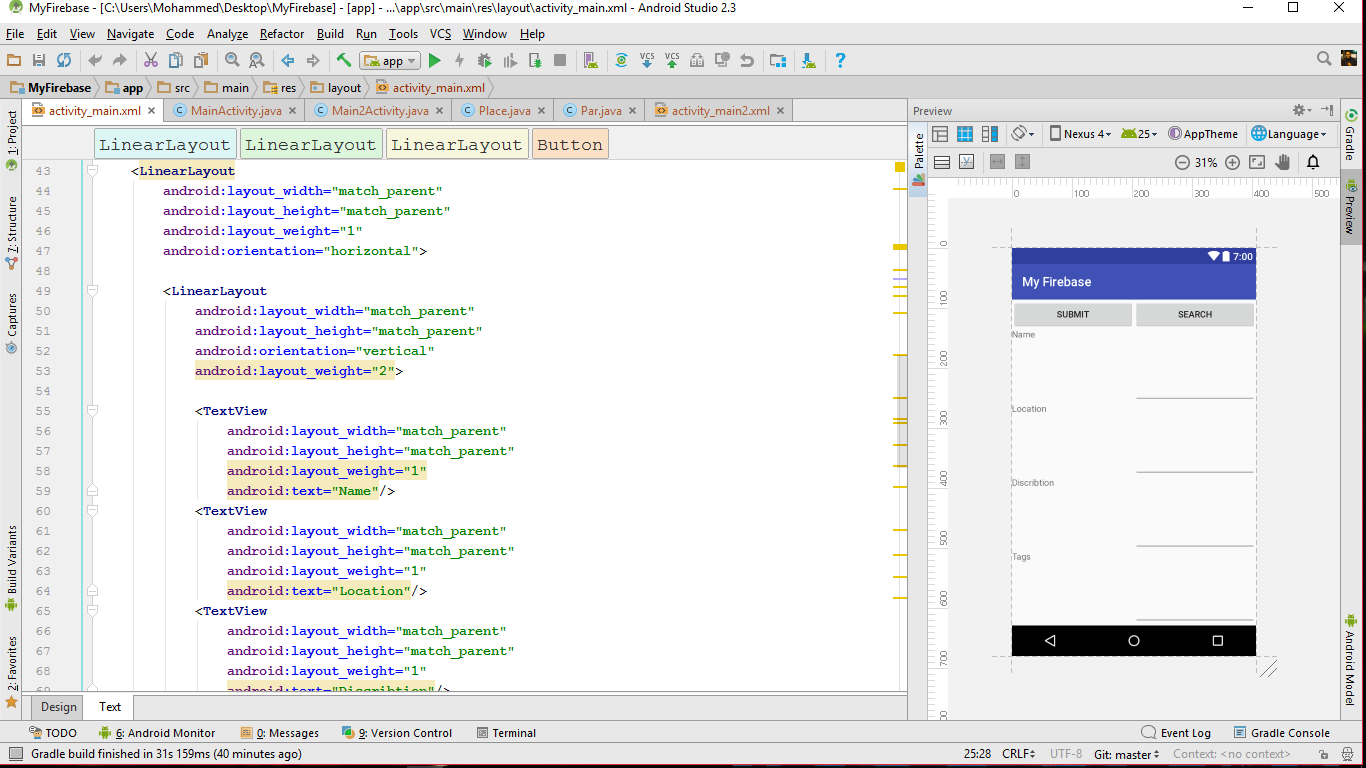
\includegraphics[height=3in]{./TeX_files/pic13}
		\caption[optional caption]{Design of layout}
		\label{Fig:Tobias}
	\end{figure}
}
\subsection{Code that Insert Data}
\subitem{
	Create Object from Database References and  set Url to my database root(Places)
	\begin{figure}[H]
		\centering
		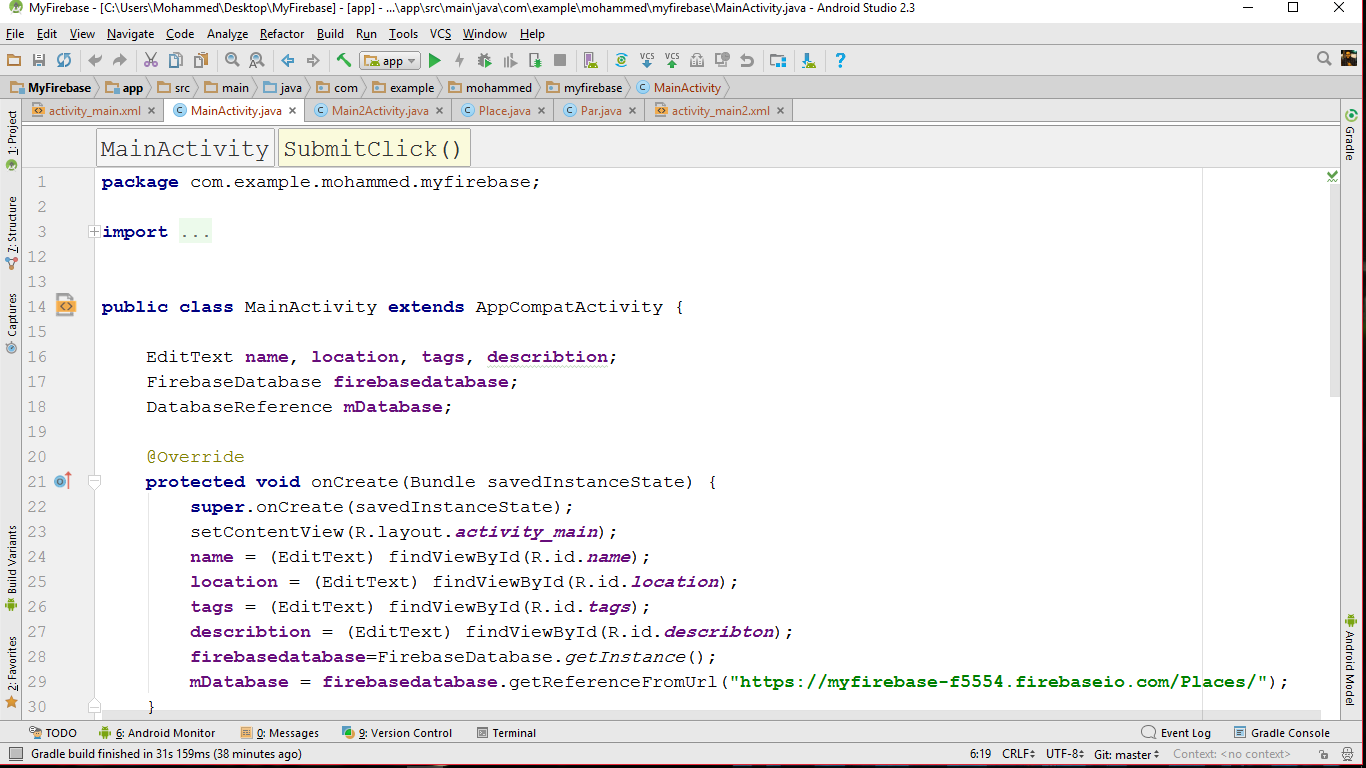
\includegraphics[height=3in]{./TeX_files/pic14}
		\caption[optional caption]{Code 1}
		\label{Fig:Tobias}
	\end{figure}
	Make Object from my Class places and set Variable to the place and push it in database back-end
	\begin{figure}[H]
		\centering
		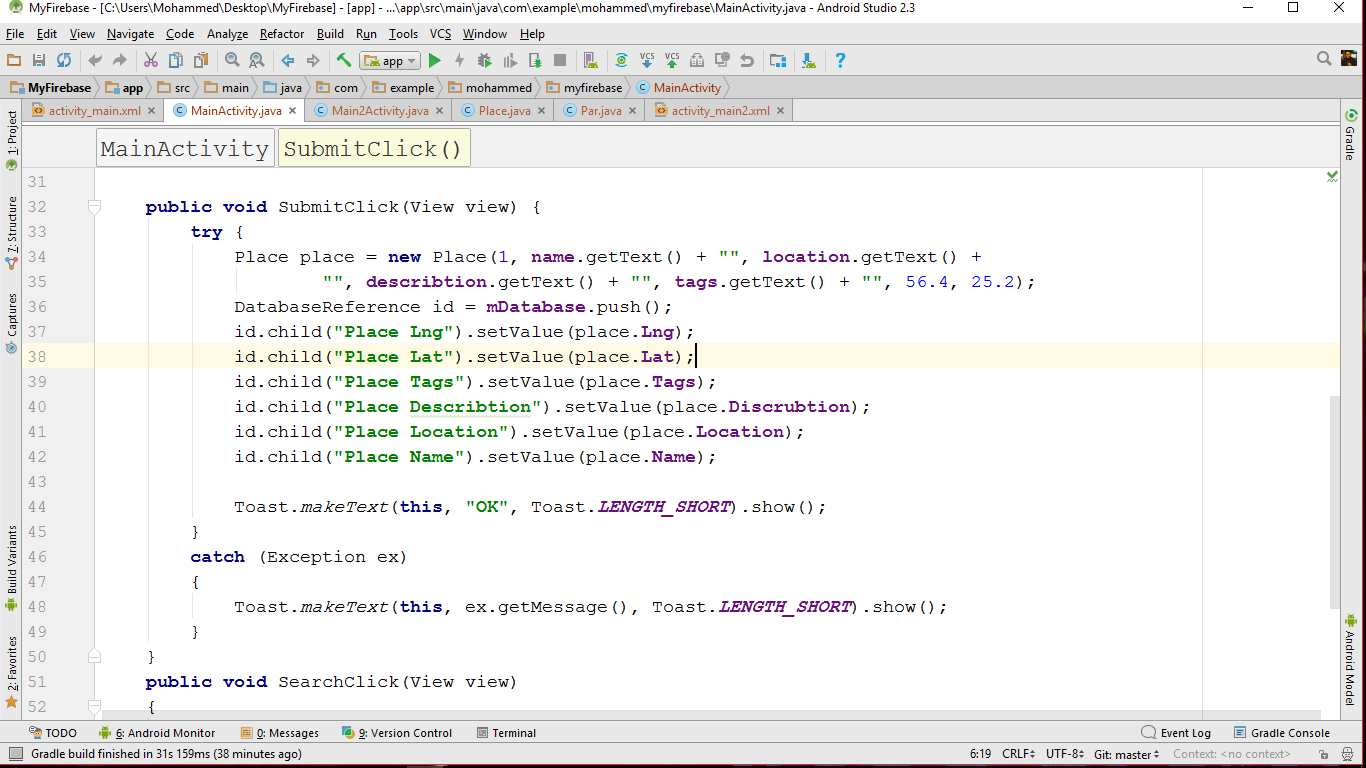
\includegraphics[height=3in]{./TeX_files/pic15}
		\caption[optional caption]{Code 2}
		\label{Fig:Tobias}
	\end{figure}
	}
\section{Retrieve Data from Firebase Back-end}
\subsection{Design Retrieve layout}
\subitem{
	\subitem{
		Retrieve data in listview and show the name of place only
		\begin{figure}[H]
			\centering
			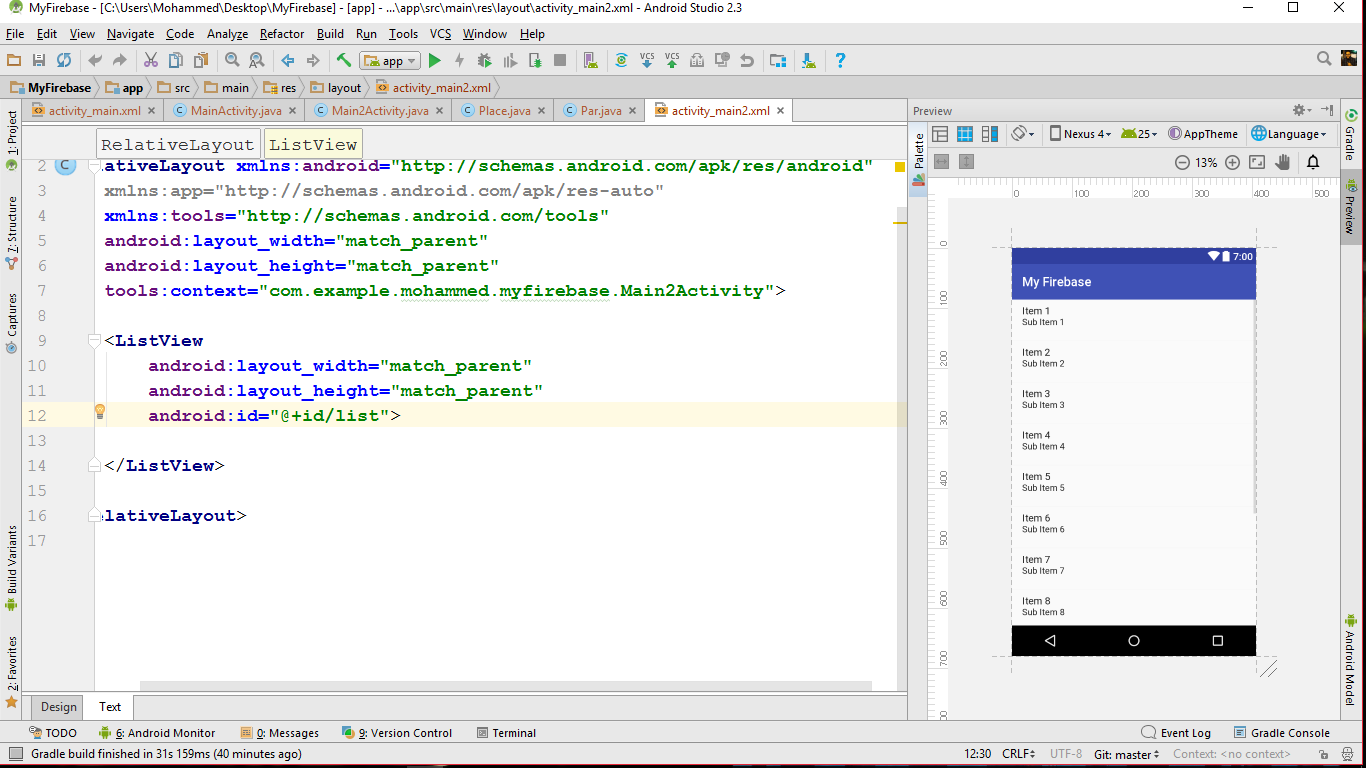
\includegraphics[height=3in]{./TeX_files/pic16}
			\caption[optional caption]{Design of layout}
			\label{Fig:Tobias}
		\end{figure}
	}
\subsection{Code that retrieve data}
\subitem{
	\subitem{
		Access To root of database (Places) and make 'For-Loob' on all child 
		\begin{figure}[H]
			\centering
			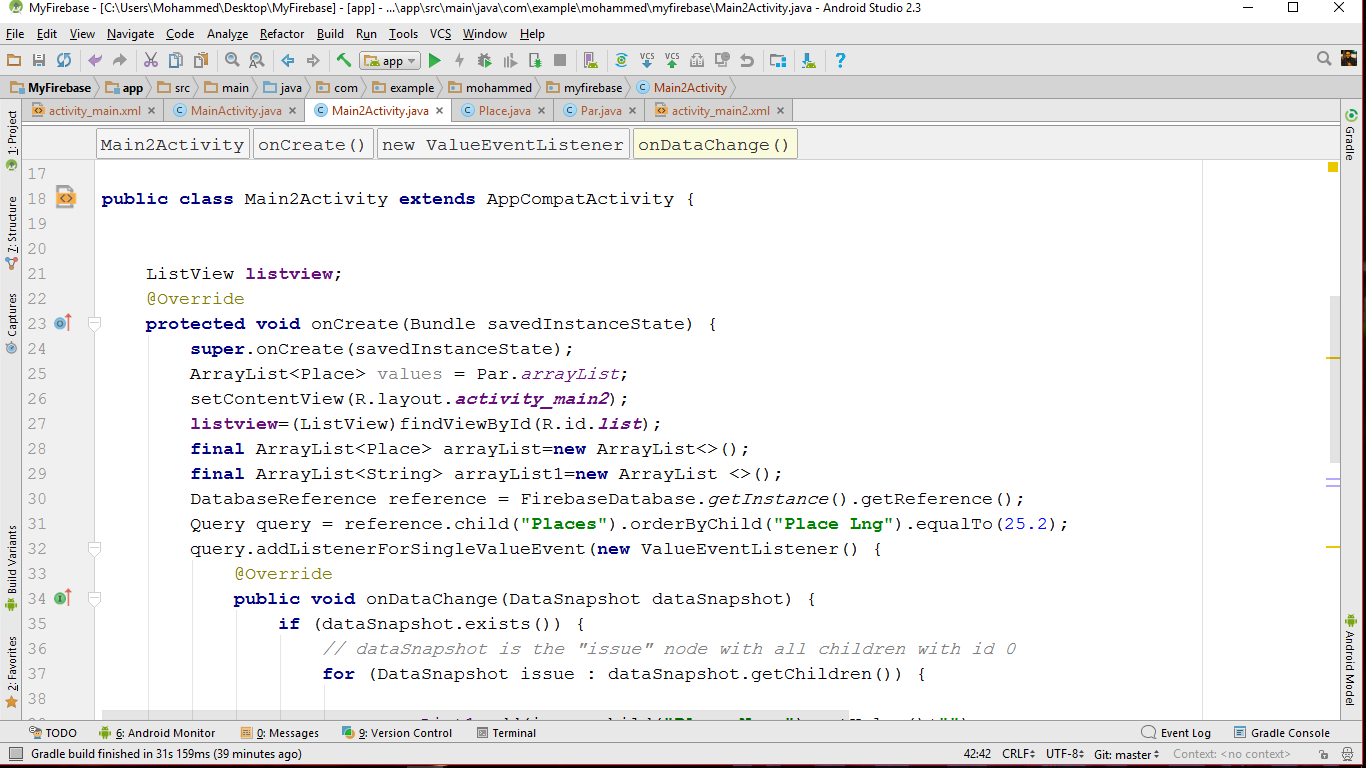
\includegraphics[height=3in]{./TeX_files/pic17}
			\caption[optional caption]{Code 1}
			\label{Fig:Tobias}
		\end{figure}
		display the name of place in listview
		\begin{figure}[H]
			\centering
			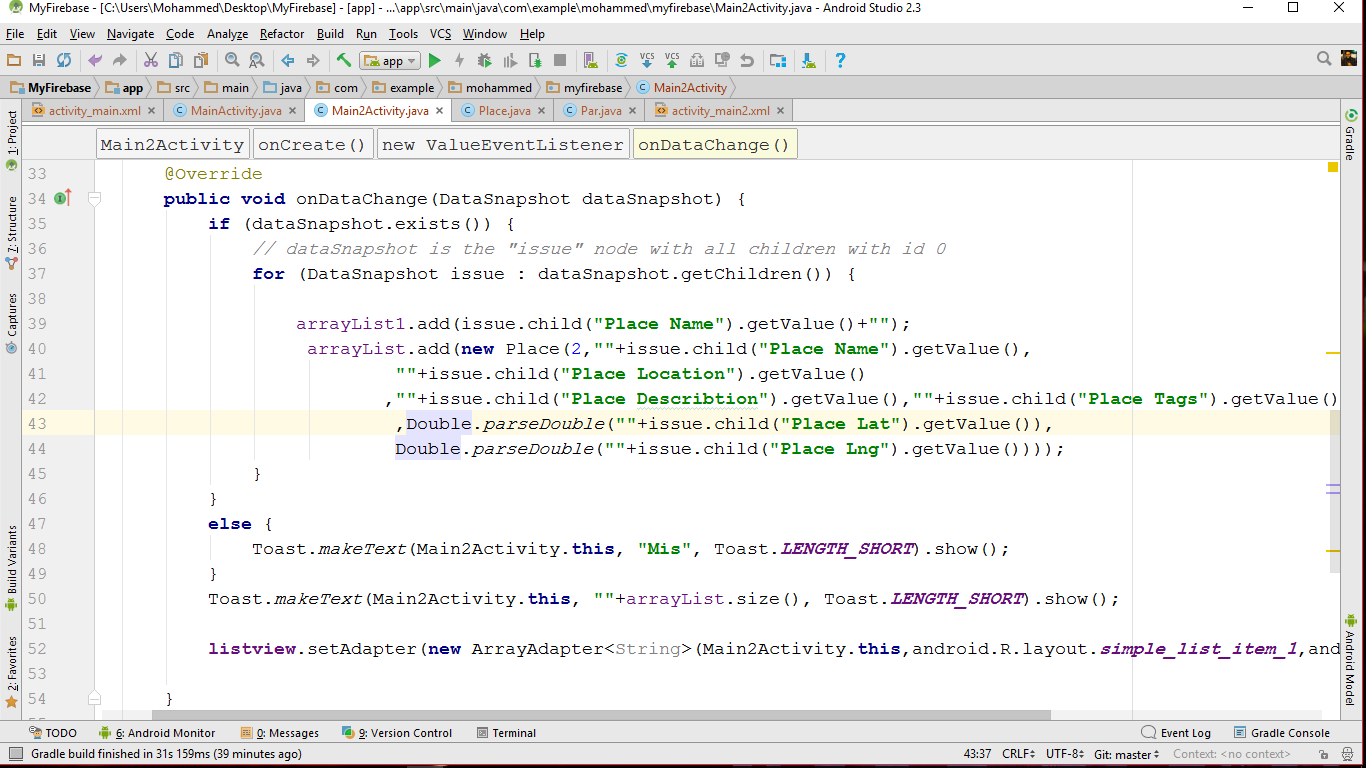
\includegraphics[height=3in]{./TeX_files/pic18}
			\caption[optional caption]{Code 2}
			\label{Fig:Tobias}
		\end{figure}
	}